\begin{question}
    Consider the experimental aircraft shown below with a vertical stabilizer located a distance $l_F$ forward of the center of gravity.
    \begin{figure}[h]
        \centering
        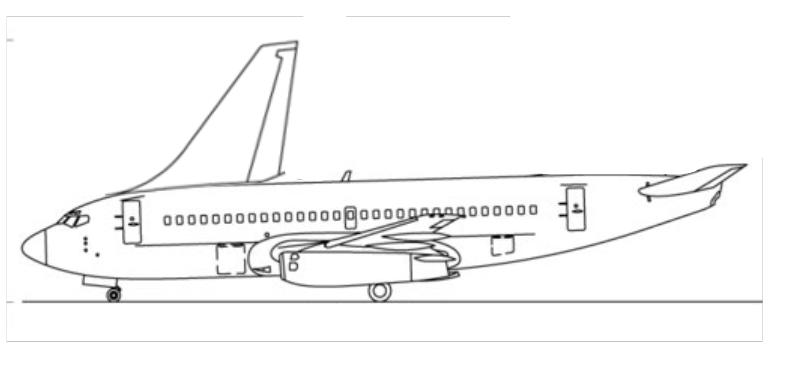
\includegraphics[width=0.65\textwidth]{figures/ForwardVStab.png}
        % \caption{}
        % \label{fig:enter-label}
    \end{figure}
    \begin{enumerate}
        \item Re-derive the yaw stiffness contribution from the vertical stabilizer, $C_{{n_F}_\beta} = \frac{\partial C_{{n_F}}}{\partial \beta}$. Let the sidewash angle, $\sigma$, and $\frac{\partial \sigma}{\partial \beta}$ be 0. Thus, $\alpha_F = -\beta$. What is the sign of $C_{{n_F}_\beta}$?
        \item Re-derive the ``rudder power" $C_{n_{\delta_r}}$.
        \item Is this a good aircraft design? Why or why not?
    \end{enumerate}
\end{question}
